\documentclass[main]{subfiles}
\begin{document}

%@@@@@@@@@@@@@@@@@@@@@@@@@@@@@@
% Main Topics: Example: The intersection of two matroids is (in general) not a
% matroid, intersection of two polymatroid polyhedra
% The intersection of two matroids - 11.12.2017
% author: Vanessa Leite

\section{The intersection of two matroids}

\subsection{The previous theorem revisited}
$(N,\mathcal{I})$ matroid, $r: 2^N \mapsto \Z_+$ submodular, non decreasing.
Consider $\max \{ \sum_{i \in N} c_i x_i \mid \sum_{i \in T} x_i \leq r(T)
\forall T \subseteq N, x_i \geq 0$, $\forall i \in N\}$. This is a integral
optimization problem, i.e., all vertices satisfying its constraints are
integral.

Consider a graph $G=(V,E)$ and the set of all forests in $G$, i.e.,
$T \subseteq E$, $(V,T)$ has no cycles.

$r(T) = |V| - z$, where $z$ is the number of components of $(V,T)$.

\subparagraph{Exercise: show that $r$ is submodular}
\todo[inline]{exercise}

Then, the $(N,\mathcal{I})$ correspondent independence system is a matroid.
Consider, $T \subseteq E$, $\sum_{i \in T} x_i \leq r(T)$ (*).\\
Assume first $(V,T)$ is connected, so (*) is $\sum_{e \in E} x_e \leq n-1$.
$-x_e \leq 0$, $\forall e \in E \setminus T$.\\
Assume now $(V,T)$ is not connected, let $(V_1, T_1), \dots, (V_k, T_k)$ be all
components of $(V,T)$. Then, (*) is dominated by inequalities:
$\sum_{e \in E(V_i)} x_e \leq |V_i| - 1 \forall i$, therefore we can describe
the original problem (find a max-weight forest).

We can walk in vertices instead of vertices: $\forall S \subseteq V$:
$\sum_{e \in E(S)} x_e \leq |S| - 1, x_e \geq 0$ (subtour elimination
constraints).\\

%In proof a theorem (lecture 23), we constructed a solution as: 
%

\paragraph{Properties of rank function}
$r(\{1, \dots, j\}) - r(\{1, \dots, j-1\}) \in \{0,1\}$, i.e, or it doesn't
change or ir increases by one. $r(\emptyset) = 0$.

Interprete the solution combinatorially. Edges are numbered $\{1, \dots, n\}$.
Take the edge with high score, if the rank increases, keep it, if not, skip it.
This is the famous greedy algorithm. It only works if we have a matroid.

\paragraph{Greedy-solution}
\begin{enumerate}
\item Sort edges $c_{e_1} \geq c_{e_2} \geq \dots \geq c_{e_k} > 0$,
$S= \emptyset$.
\item For $j = 1, \dots, k$:
\subitem if $(V,S\cup \{e_j\})$ does not create a cycle, then, $S = S \cup
\{e_j\}$
\item return S
\end{enumerate}

\paragraph{Remark: In lecture 19, we introduced two formulation for the mininum
spanning tree problem}
$G=(V,E)$ connected, $P_{cut} \supseteq P_{SUB}$, $|V| = n$, $|E| = m$.
$P_{SUB} = \{x \geq 0 \mid \sum_{e \in E} x_e = n-1,
\sum_{e \in E(S)} x_e \leq |S| -1 \forall S \subseteq V\}$.

\paragraph{Claim: $P_{SUB}$ is integral}
$Q = \{x \geq 0 \mid \sum_{e \in E(S)} x_e \leq |S|-1, \forall S \subseteq V\}$
is integral. $Q \cap \{x: \sum_{e \in E} x_e = n-1\}$ is integral. For all
points $x \in Q$ then $\sum_{e \in E} x_e \leq n-1$.
$F = \{x \in Q \mid \sum_{e \in E} x_e = n-1\}$ is a face of $Q \rightarrow F$
is integral $\rightarrow P_{SUB}$ is integral.

\subsection{The intersection of two matroids theorem}
$(N,\mathcal{I})$ is an independence system. $\mathcal{I} = \mathcal{I}_1
\cap \mathcal{I}_2$, where $(N,\mathcal{I}_i)$ are matroids.

\paragraph{Example:}
$D=(V,A)$ a digraph. $T \subseteq A$ is a branching if $(V,T)$ contains no
cycle and $\forall v \in V$: $\abs{\delta^-(v) \cap T} \leq 1$.
Greedy algorithm does not work.
\begin{figure}[!h]
  \centering
    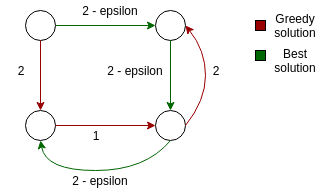
\includegraphics[width=0.3\textwidth]{imgs/matroid-intersection.png}
\end{figure}

$\mathcal{I}_1 = \{ T \subseteq A \mid |\delta^-(v) \cap T | \leq 1,
\forall v \in V\}$ (partition matroid)
$\mathcal{I}_2 = \{ T \subseteq A \mid (V,T) \text{ no cycle }\}$ (graphic
matroid)
$\mathcal{I} = \mathcal{I_1} \cap \mathcal{I_2}$.

Consider optimization problem over intersection of two matroids:\\
$Z = \max \{\sum_{j=1}^n c_j x_j \mid$
$\underbrace{\sum_{j \in T} x_j \leq min\{r_1(T), r_2(T)\} \forall T \subseteq
N, x \geq 0}_{P} \}$, where $r_i$ are rank functions of the two matroids.

Task: find $x \in P \cap \Z^n$.

\paragraph{Theorem: $r_i$ are submodular, integer valued, $r_i (\emptyset) =
0$, $r_i$ non decreasing, then $P$ is integral.}
\subparagraph{Proof:}
$\forall c \in \Z^n$, then $z \in \Z \rightarrow P$ is integral.

\paragraph{The dual for $\displaystyle \max_{x \in P} c^T x$ is}
$\min \{\sum_{S \subseteq N} r_1(S) y_i(S) + \sum_{S \subseteq N} r_2(S) +
y_2(S) \mid$
$\sum_{s: j \in S} y_1(s) + \sum_{s: j \in S} y_2(s) \geq c_j \forall j \in N,
y_i(s) \geq 0 \}$ (*)

Let $(y^*_1, y^*_2)$ be an optimal dual solution. Let $c_{ji} = \sum_{s: j \in 
S} y_i^*(s)$ for $i = 1,2, j \in N$.

Consider: $\min \sum_{s: j \in S} r_i(S) y_i(S)$, for $i=1,2$ st
$\underbrace{\sum_{s:j\in S} y_i(S) \geq c_{ji} \forall j \in N, y_i(s) \geq 0,
\forall S}_{D_i}$.

$\min \sum r_i(S) y_i(S)$, $y_i \in D$ is a dual matroid optimization problem.

From the proof of previou theorem, there exists an alternative dual optimal
solution $\bar{y_i}(S), \forall S$ st $\{s: \bar{y_1}(S) > 0 \} = \{S_1 \subset
S_2 \subset \dots \subset S_k\}$, $\{s: \bar{y_2}(S) > 0 \} = \{U_1 \subset U_2
\subset \dots \subset U_r\}$.\\
Thus, there exists an alternative opt. solution $(y_1, y_2)$ for the dual (*)
that satisfies:\\
$Z^{**} = \min \sum_{j=1}^k r_1(S_j) y_1(S_j) + \sum_{j=1}^r r_2(U_j) y_2(U_j)$
st $B y \geq c, y \geq 0$ (**), where $B$ is a matrix with $k+r$ columns. 
$B_{ij} = 1$ if $i \in S_j$.
$j \geq k+1$, $B_{ij} \in \{0,1\}$, $B_{ij} = 1$ if $i \in U_{r + 1 - (j-k)}$
(reverse order).

(**) is a restricted system for (*) by setting many $y_i(S) = 0$.
In every row of $B$, the $1$-entries come consecutively. So, this matrix $B$ is
TU. $c$ is integral, $r_i(S)$ is also integral $\rightarrow y$ optimal for (**)
is integral $\rightarrow Z^{**}$ is integral $\forall c \in \Z^n$.

\end{document}